\section{Appendix}

% %table%
% \begin{table}
% \centering
% \caption{Probabilities for Gender (G)}\label{tab1}
% \begin{tabular}{|l|l|}
% \hline
% G &  P\\
% \hline
% F &	0.51\\
% T &	0.49\\
% \hline
% \end{tabular}
% \end{table}

% %table%
% \begin{table}
% \centering
% \caption{Probabilities for job-type (JT)}\label{tab1}
% \begin{tabular}{|l|l|}
% \hline
% JT &  P\\
% \hline
% F &	0.65\\
% T &	0.35\\
% \hline
% \end{tabular}
% \end{table}

% %table%
% \begin{table}
% \centering
% \caption{Probabilities for high job demands (HJD)}\label{tab1}
% \begin{tabular}{|l|l|l|l|}
% \hline
% JT & G & HJD & HJD $\mid$ JT, G \\
% \hline
% F &	F &	F &	0.44\\
% F &	F &	T &	0.55\\
% F &	T &	F &	0.45\\
% F &	T &	T &	0.55\\
% T &	F &	F &	0.61\\
% T &	F &	T &	0.39\\
% T &	T &	F &	0.22\\
% T &	T &	T &	0.78\\
% \hline
% \end{tabular}
% \end{table}

% \begin{table}
% \centering
% \caption{Probabilities for low decision latitude (LDL)}\label{tab1}
% \begin{tabular}{|l|l|l|l|}
% \hline
% JT &  G & LDL & LDL $\mid$ JT, G\\
% \hline
% F &	F &	F &	0.21\\
% F &	F &	T &	0.79\\
% F &	T &	F &	0.41\\
% F &	T &	T &	0.59\\
% T &	F &	F &	0.63\\
% T &	F &	T &	0.27\\
% T &	T &	F &	0.67\\
% T &	T &	T &	0.33\\
% \hline
% \end{tabular}
% \end{table}


% %table%
% \begin{table}
% \centering
% \caption{Probabilities for low income (LI)}\label{tab1}
% \begin{tabular}{|l|l|l|l|}
% \hline
% JT & G &  LI & LI $\mid$ JT, G \\
% \hline
% F &	F &	F &	0.2\\
% F &	F &	T &	0.8\\
% F &	T &	F &	0.31\\
% F &	T &	T &	0.69\\
% T &	F &	F &	0.63\\
% T &	F &	T &	0.37\\
% T &	T &	F &	0.59\\
% T &	T &	T &	0.41\\

% \hline
% \end{tabular}
% \end{table}

% \begin{table}
% \centering
% \caption{Probabilities for restricted social opportunities (RSO)}\label{tab1}
% \begin{tabular}{|l|l|l|l|}
% \hline
% HJD & LI & RSO & RSO $\mid$ HJD, LI\\
% \hline
% F &	F &	F &	0.74\\
% F &	F &	T &	0.26\\
% F &	T &	F &	0.3\\
% F &	T &	T &	0.7\\
% T &	F &	F &	0.34\\
% T &	F &	T &	0.66\\
% T &	T &	F &	0.18\\
% T &	T &	T &	0.82\\
% \hline
% \end{tabular}
% \end{table}


% \begin{table}
% \centering
% \caption{Probabilities for Occupational strain (OS)}\label{tab1}
% \begin{tabular}{|l|l|l|l|l|l|l|}
% \hline
% LDL & HJD & LI & RSO & OS & OS $\mid$ LDL, HJD, LI, RSO\\
% \hline
% F &	F &	F &	F &	F &	0.95\\
% F &	F &	F&	F &	T &	0.05\\
% F &	F &	F &	T &	F &	0.31\\
% F & F &	F &	T &	T &	0.69\\
% F &	F &	T &	F &	F &	0.22\\
% F &	F &	T &	F &	T &	0.78\\
% F &	F & T &	T &	F &	0.2\\
% F &	F &	T &	T &	T &	0.8\\
% F &	T &	F &	F &	F &	0.21\\
% F & T &	F &	F &	T &	0.79\\
% F &	T &	F &	T &	F &	0.17\\
% F &	T &	F &	T &	T &	0.83\\
% F &	T &	T &	F &	F &	0.33\\
% F &	T &	T &	F &	T &	0.67\\
% F &	T &	T &	T &	F &	0.35\\
% F & T &	T &	T &	T & 	0.65\\
% T &	F &	F &	F &	F &	0.25\\
% T &	F &	F &	F &	T &	0.75\\
% T & 	F &	F &	T &	F &	0.32\\
% T &	F &	F &	T &	T &	0.68\\
% T &	F &	T &	F &	F &	0.22\\
% T &	F &	T &	F &	T & 	0.78\\
% T & 	F &	T &	T &	F &	0.29\\
% T &	F &	T &	T &	T &	0.71\\
% T &	T &	F &	F &	F &	0.31\\
% T &	T &	F &	F &	T & 	0.69\\
% T &	T &	F &	T &	F &	0.27\\
% T &	T &	F &	T &	T &	0.73\\
% T &	T &	T &	F &	F &	0.22\\
% T &	T &	T &	F &	T &	0.78\\
% T &	T &	T &	T &	F &	0.11\\
% T &	T &	T &	T &	T &	0.89\\

% \hline
% \end{tabular}
% \end{table}

% %table%
% \begin{table}
% \centering
% \caption{Probabilities for Mobbing (M)}\label{tab1}
% \begin{tabular}{|l|l|}
% \hline
% M &  P\\
% \hline
% F &	0.6\\
% T &	0.4\\
% \hline
% \end{tabular}
% \end{table}


% \begin{table}
% \centering
% \caption{Probabilities for job burnout (JB))}\label{tab1}
% \begin{tabular}{|l|l|l|l|}
% \hline
% OS & M & JB & JB $\mid$ OS, M\\
% \hline
% F &	F &	F &	0.8\\
% F &	F &	T &	0.2\\
% F &	T &	F &	0.22\\
% F &	T &	T &	0.78\\
% T &	F &	F &	0.2\\
% T &	F &	T &	0.8\\
% T &	T &	F &	0.05\\
% T &	T &	T &	0.95\\
% \hline
% \end{tabular}
% \end{table}

% \begin{table}
% \centering
% \caption{Probabilities for high cholesterol (HC))}\label{tab1}
% \begin{tabular}{|l|l|l|l|}
% \hline
% OS & JB & HC & HC $\mid$ OS, JB\\
% \hline
% F &	F &	F &	0.56\\
% F &	F &	T &	0.44\\
% F &	T &	F &	0.15\\
% F &	T &	T &	0.85\\
% T &	F &	F &	0.3\\
% T &	F &	T &	0.7\\
% T &	T &	F &	0.27\\
% T &	T &	T &	0.73\\
% \hline
% \end{tabular}
% \end{table}


% \begin{table}
% \centering
% \caption{Probabilities for smoking (S))}\label{tab1}
% \begin{tabular}{|l|l|l|l|}
% \hline
% OS & JB & S & S $\mid$ OS, JB\\
% \hline
% F &	F &	F &	0.55\\
% F &	F &	T &	0.45\\
% F &	T &	F &	0.2\\
% F &	T &  T &	0.8\\
% T &	F &	F &	0.31\\
% T &	F &	T &	0.69\\
% T &	T &	F &	0.25\\
% T &	T &	T &	0.75\\
% \hline
% \end{tabular}
% \end{table}




% \begin{table}
% \centering
% \caption{Probabilities for hypertension (H)}\label{tab1}
% \begin{tabular}{|l|l|l|l|}
% \hline
% OS & JB & H & H $\mid$ OS, JB\\
% \hline
% F &	F &	F &	0.61\\
% F &	F &	T &	0.39\\
% F &	T &	F &	0.32\\
% F &	T &	T &	0.68\\
% T &	F &	F &	0.25\\
% T &	F &	T &	0.75\\
% T &	T &	F &	0.16\\
% T &	T &	T &	0.84\\
% \hline
% \end{tabular}
% \end{table}

% \begin{table}
% \centering
% \caption{Probabilities for Lung Cancer (LC)}\label{tab1}
% \begin{tabular}{|l|l|l|l|}
% \hline
%  HC & S & LS & LC $\mid$ HC, S\\
% \hline
% F &	F &	F &	0.71\\
% F &	F &	T &	0.29\\
% F &	T &	F &	0.25\\
% F &	T &	T &	0.75\\
% T &	F &	F &	0.37\\
% T &	F &	T &	0.63\\
% T &	T &	F &	0.11\\
% T &	T &	T &	0.89\\
% \hline
% \end{tabular}
% \end{table}

% \begin{table}
% \centering
% \caption{Probabilities for coronary heart disease (CHD)}\label{tab1}
% \begin{tabular}{|l|l|l|l|l|l|}
% \hline
% HC & S & H & OS & CHD & CHD $\mid$ HC, S, H, OS, CHD\\
% \hline
% F &	F &	F &	F &	F &	0.84\\
% F &	F &	F &	F &	T &	0.16\\
% F &	F &	T &	F &	F &	0.42\\
% F &	F &	T &	F &	T &	0.58\\
% F &	F &	F &	T &	F &	0.62\\
% F &	F &	F &	T &	T &	0.38\\
% F &	F &	T &	T &	F &	0.38\\
% F &	F &	T &	T &	T &	0.62\\
% F &	T &	F &	T & 	F &	0.25\\
% F &	T &	F &	F &	F &	0.53\\
% F &	T &	F &	F &	T &	0.47\\
% F &	T &	T &	F &	F &	0.11\\
% F &	T &	T &	F &	T &	0.89\\
% F &	T &	F &	T &	T &	0.75\\
% F &	T &	T &	T &	F &	0.33\\
% F &	T &	T &	T &	T &	0.67\\
% T &	F &	F &	F &	F &	0.46\\
% T &	F &	F &	F &	T &	0.54\\
% T &	F &	T &	F &	F &	0.66\\
% T &	F &	T &	F &	T &	0.34\\
% T &	F &	F &	T &	F &	0.65\\
% T &	F &	F &	T &	T &	0.35\\
% T &	F &	T &	T & F &	0.58\\
% T &	F &	T &	T &	T &	0.42\\
% T &	T &	F & F &	F &	0.32\\
% T &	T &	F &	F &	T &	0.68\\
% T &	T &	T &	F &	F &	0.44\\
% T &	T &	T &  F &	T &	0.56\\
% T &	T &	F &	T &	F &	0.24\\
% T &	T &	F & T &	T &	0.76\\
% T &	T &  T &	T &	F &	0.04\\
% T &	T &	T &	T &	T &	0.96\\
% \hline
% \end{tabular}
% \end{table}


\begin{figure}[H]
    %\centering
    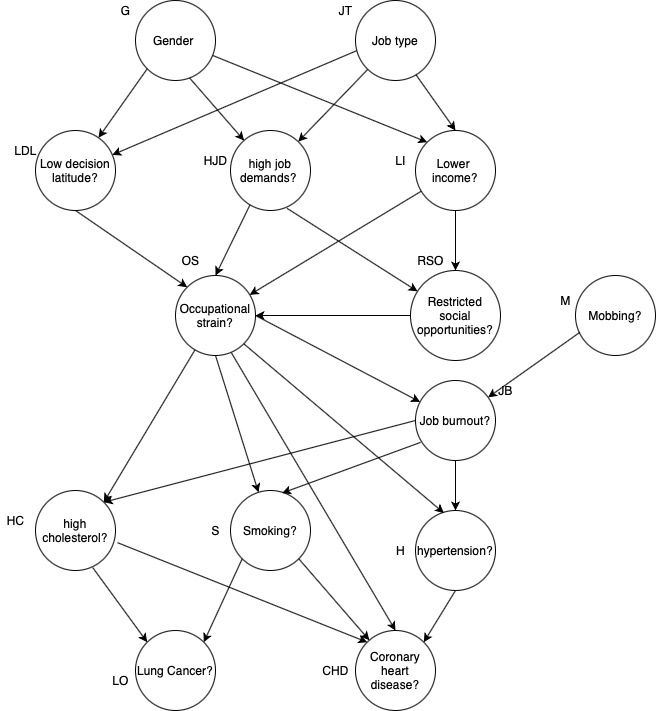
\includegraphics[width= 1.2\textwidth]{Assets/BN_diseases.jpg}
    \caption{BN of the use case}
    \label{fig:my_label}
\end{figure}

%table%
\begin{table}
\centering
\caption{Probabilities for Gender (G)}\label{tab1}
\begin{tabular}{p{1.2cm} p{1.2cm} }
\hline
G &  P\\
\hline
F &	0.51\\
T &	0.49\\
\hline
\end{tabular}
\end{table}

%table%
\begin{table}
\centering
\caption{Probabilities for job-type (JT)}\label{tab1}
\begin{tabular}{p{1.2cm} p{1.2cm} }
\hline
JT &  P\\
\hline
F &	0.65\\
T &	0.35\\
\hline
\end{tabular}
\end{table}

%table%
\begin{table}
\centering
\caption{Probabilities for high job demands (HJD)}\label{tab1}
\begin{tabular}{p{1.2cm} p{1.2cm} p{1.2cm} p{1.5cm} }
\hline
JT & G & HJD & HJD $\mid$ JT, G \\
\hline
F &	F &	F &	0.44\\
F &	F &	T &	0.55\\
F &	T &	F &	0.45\\
F &	T &	T &	0.55\\
T &	F &	F &	0.61\\
T &	F &	T &	0.39\\
T &	T &	F &	0.22\\
T &	T &	T &	0.78\\
\hline
\end{tabular}
\end{table}

\begin{table}
\centering
\caption{Probabilities for low decision latitude (LDL)}\label{tab1}
\begin{tabular}{p{1.2cm} p{1.2cm} p{1.2cm} p{1.5cm} }
\hline
JT &  G & LDL & LDL $\mid$ JT, G\\
\hline
F &	F &	F &	0.21\\
F &	F &	T &	0.79\\
F &	T &	F &	0.41\\
F &	T &	T &	0.59\\
T &	F &	F &	0.63\\
T &	F &	T &	0.27\\
T &	T &	F &	0.67\\
T &	T &	T &	0.33\\
\hline
\end{tabular}
\end{table}


%table%
\begin{table}
\centering
\caption{Probabilities for low income (LI)}\label{tab1}
\begin{tabular}{p{1.2cm} p{1.2cm} p{1.2cm} p{1.5cm} }
\hline
JT & G &  LI & LI $\mid$ JT, G \\
\hline
F &	F &	F &	0.2\\
F &	F &	T &	0.8\\
F &	T &	F &	0.31\\
F &	T &	T &	0.69\\
T &	F &	F &	0.63\\
T &	F &	T &	0.37\\
T &	T &	F &	0.59\\
T &	T &	T &	0.41\\

\hline
\end{tabular}
\end{table}

\begin{table}
\centering
\caption{Probabilities for restricted social opportunities (RSO)}\label{tab1}
\begin{tabular}{p{1.2cm} p{1.2cm} p{1.2cm} p{2.5cm} }
\hline
HJD & LI & RSO & RSO $\mid$ HJD, LI\\
\hline
F &	F &	F &	0.74\\
F &	F &	T &	0.26\\
F &	T &	F &	0.3\\
F &	T &	T &	0.7\\
T &	F &	F &	0.34\\
T &	F &	T &	0.66\\
T &	T &	F &	0.18\\
T &	T &	T &	0.82\\
\hline
\end{tabular}
\end{table}


\begin{table}
\centering
\caption{Probabilities for Occupational strain (OS)}\label{tab1}
\begin{tabular}{p{1.2cm} p{1.2cm} p{1.2cm} p{1.2cm} p{1.2cm} p{2cm} }
\hline
LDL & HJD & LI & RSO & OS & OS $\mid$ LDL, HJD, LI, RSO\\
\hline
F &	F &	F &	F &	F &	0.95\\
F &	F &	F&	F &	T &	0.05\\
F &	F &	F &	T &	F &	0.31\\
F & F &	F &	T &	T &	0.69\\
F &	F &	T &	F &	F &	0.22\\
F &	F &	T &	F &	T &	0.78\\
F &	F & T &	T &	F &	0.2\\
F &	F &	T &	T &	T &	0.8\\
F &	T &	F &	F &	F &	0.21\\
F & T &	F &	F &	T &	0.79\\
F &	T &	F &	T &	F &	0.17\\
F &	T &	F &	T &	T &	0.83\\
F &	T &	T &	F &	F &	0.33\\
F &	T &	T &	F &	T &	0.67\\
F &	T &	T &	T &	F &	0.35\\
F & T &	T &	T &	T & 	0.65\\
T &	F &	F &	F &	F &	0.25\\
T &	F &	F &	F &	T &	0.75\\
T & 	F &	F &	T &	F &	0.32\\
T &	F &	F &	T &	T &	0.68\\
T &	F &	T &	F &	F &	0.22\\
T &	F &	T &	F &	T & 	0.78\\
T & 	F &	T &	T &	F &	0.29\\
T &	F &	T &	T &	T &	0.71\\
T &	T &	F &	F &	F &	0.31\\
T &	T &	F &	F &	T & 	0.69\\
T &	T &	F &	T &	F &	0.27\\
T &	T &	F &	T &	T &	0.73\\
T &	T &	T &	F &	F &	0.22\\
T &	T &	T &	F &	T &	0.78\\
T &	T &	T &	T &	F &	0.11\\
T &	T &	T &	T &	T &	0.89\\

\hline
\end{tabular}
\end{table}

%table%
\begin{table}
\centering
\caption{Probabilities for Mobbing (M)}\label{tab1}
\begin{tabular}{p{1.2cm} p{1.2cm} }
\hline
M &  P\\
\hline
F &	0.6\\
T &	0.4\\
\hline
\end{tabular}
\end{table}


\begin{table}
\centering
\caption{Probabilities for job burnout (JB))}\label{tab1}
\begin{tabular}{p{1.2cm} p{1.2cm} p{1.2cm} p{2cm} }
\hline
OS & M & JB & JB $\mid$ OS, M\\
\hline
F &	F &	F &	0.8\\
F &	F &	T &	0.2\\
F &	T &	F &	0.22\\
F &	T &	T &	0.78\\
T &	F &	F &	0.2\\
T &	F &	T &	0.8\\
T &	T &	F &	0.05\\
T &	T &	T &	0.95\\
\hline
\end{tabular}
\end{table}

\begin{table}
\centering
\caption{Probabilities for high cholesterol (HC))}\label{tab1}
\begin{tabular}{p{1.2cm} p{1.2cm} p{1.2cm} p{2cm} }
\hline
OS & JB & HC & HC $\mid$ OS, JB\\
\hline
F &	F &	F &	0.56\\
F &	F &	T &	0.44\\
F &	T &	F &	0.15\\
F &	T &	T &	0.85\\
T &	F &	F &	0.3\\
T &	F &	T &	0.7\\
T &	T &	F &	0.27\\
T &	T &	T &	0.73\\
\hline
\end{tabular}
\end{table}


\begin{table}
\centering
\caption{Probabilities for smoking (S))}\label{tab1}
\begin{tabular}{p{1.2cm} p{1.2cm} p{1.2cm} p{2.2cm} }
\hline
OS & JB & S & S $\mid$ OS, JB\\
\hline
F &	F &	F &	0.55\\
F &	F &	T &	0.45\\
F &	T &	F &	0.2\\
F &	T &  T &	0.8\\
T &	F &	F &	0.31\\
T &	F &	T &	0.69\\
T &	T &	F &	0.25\\
T &	T &	T &	0.75\\
\hline
\end{tabular}
\end{table}




\begin{table}
\centering
\caption{Probabilities for hypertension (H)}\label{tab1}
\begin{tabular}{p{1.2cm} p{1.2cm} p{1.2cm} p{2cm} }
\hline
OS & JB & H & H $\mid$ OS, JB\\
\hline
F &	F &	F &	0.61\\
F &	F &	T &	0.39\\
F &	T &	F &	0.32\\
F &	T &	T &	0.68\\
T &	F &	F &	0.25\\
T &	F &	T &	0.75\\
T &	T &	F &	0.16\\
T &	T &	T &	0.84\\
\hline
\end{tabular}
\end{table}

\begin{table}
\centering
\caption{Probabilities for Lung Cancer (LC)}\label{tab1}
\begin{tabular}{p{1.2cm} p{1.2cm} p{1.2cm} p{2cm} }
\hline
 HC & S & LS & LC $\mid$ HC, S\\
\hline
F &	F &	F &	0.71\\
F &	F &	T &	0.29\\
F &	T &	F &	0.25\\
F &	T &	T &	0.75\\
T &	F &	F &	0.37\\
T &	F &	T &	0.63\\
T &	T &	F &	0.11\\
T &	T &	T &	0.89\\
\hline
\end{tabular}
\end{table}

\begin{table}
\centering
\caption{Probabilities for coronary heart disease (CHD)}\label{tab1}
\begin{tabular}{p{1.2cm} p{1.2cm} p{1.2cm} p{1.2cm} p{1.2cm} p{2cm} }
\hline
HC & S & H & OS & CHD & CHD $\mid$ HC, S, H, OS, CHD\\
\hline
F &	F &	F &	F &	F &	0.84\\
F &	F &	F &	F &	T &	0.16\\
F &	F &	T &	F &	F &	0.42\\
F &	F &	T &	F &	T &	0.58\\
F &	F &	F &	T &	F &	0.62\\
F &	F &	F &	T &	T &	0.38\\
F &	F &	T &	T &	F &	0.38\\
F &	F &	T &	T &	T &	0.62\\
F &	T &	F &	T & 	F &	0.25\\
F &	T &	F &	F &	F &	0.53\\
F &	T &	F &	F &	T &	0.47\\
F &	T &	T &	F &	F &	0.11\\
F &	T &	T &	F &	T &	0.89\\
F &	T &	F &	T &	T &	0.75\\
F &	T &	T &	T &	F &	0.33\\
F &	T &	T &	T &	T &	0.67\\
T &	F &	F &	F &	F &	0.46\\
T &	F &	F &	F &	T &	0.54\\
T &	F &	T &	F &	F &	0.66\\
T &	F &	T &	F &	T &	0.34\\
T &	F &	F &	T &	F &	0.65\\
T &	F &	F &	T &	T &	0.35\\
T &	F &	T &	T & F &	0.58\\
T &	F &	T &	T &	T &	0.42\\
T &	T &	F & F &	F &	0.32\\
T &	T &	F &	F &	T &	0.68\\
T &	T &	T &	F &	F &	0.44\\
T &	T &	T &  F &	T &	0.56\\
T &	T &	F &	T &	F &	0.24\\
T &	T &	F & T &	T &	0.76\\
T &	T &  T &	T &	F &	0.04\\
T &	T &	T &	T &	T &	0.96\\
\hline
\end{tabular}
\end{table}